\chapter{INTRODUCTION}

The need for creating an autonomous underwater vehicle surfaced when the Distributed Robotic Exploration and Mapping Systems (DREAMS) Lab became a part of the Center for Global Discovery and Conservation Science (GDCS) at Arizona State University (ASU). DREAMS has experience building and deploying autonomous systems that aid in scientific studies. These systems are typically unmanned aerial vehicles (UAV) or drones, but boats and submersibles are also in operations. GDCS participates in a range of conservation sciences, but one of their main focuses is on imaging, both in the visible spectrum and beyond. Ecologically, they have focused on rain forests and coral reefs, among other biomes. Considering the capabilities of DREAMS and the needs of GDCS for methods of imaging and exploring coral reefs, the idea of building an underwater vehicle was born.

Autonomous Underwater Vehicles (AUV) and Remotely Operated Vehicles (ROV) have been exploring the oceans for decades. However, many of these vehicles have drawbacks and limitations. ROVs are typically used when precision control and navigation of close quarters are needed. To accomplish this they require an experienced operator on the surface connected to the vehicle via a tether. The need for a tether limits where ROVs can go and who can deploy them. AUVs run autonomously, not needing a tether or operator. They are typically used in open ocean environments, where there are no obstacles or impediments to following a predetermined flight path. Making matters more difficult, most commercially available ROVs and AUVs come with proprietary software systems, limiting the ability to use state-of-the-art autonomous navigation tools. 

\begin{figure}[ht]
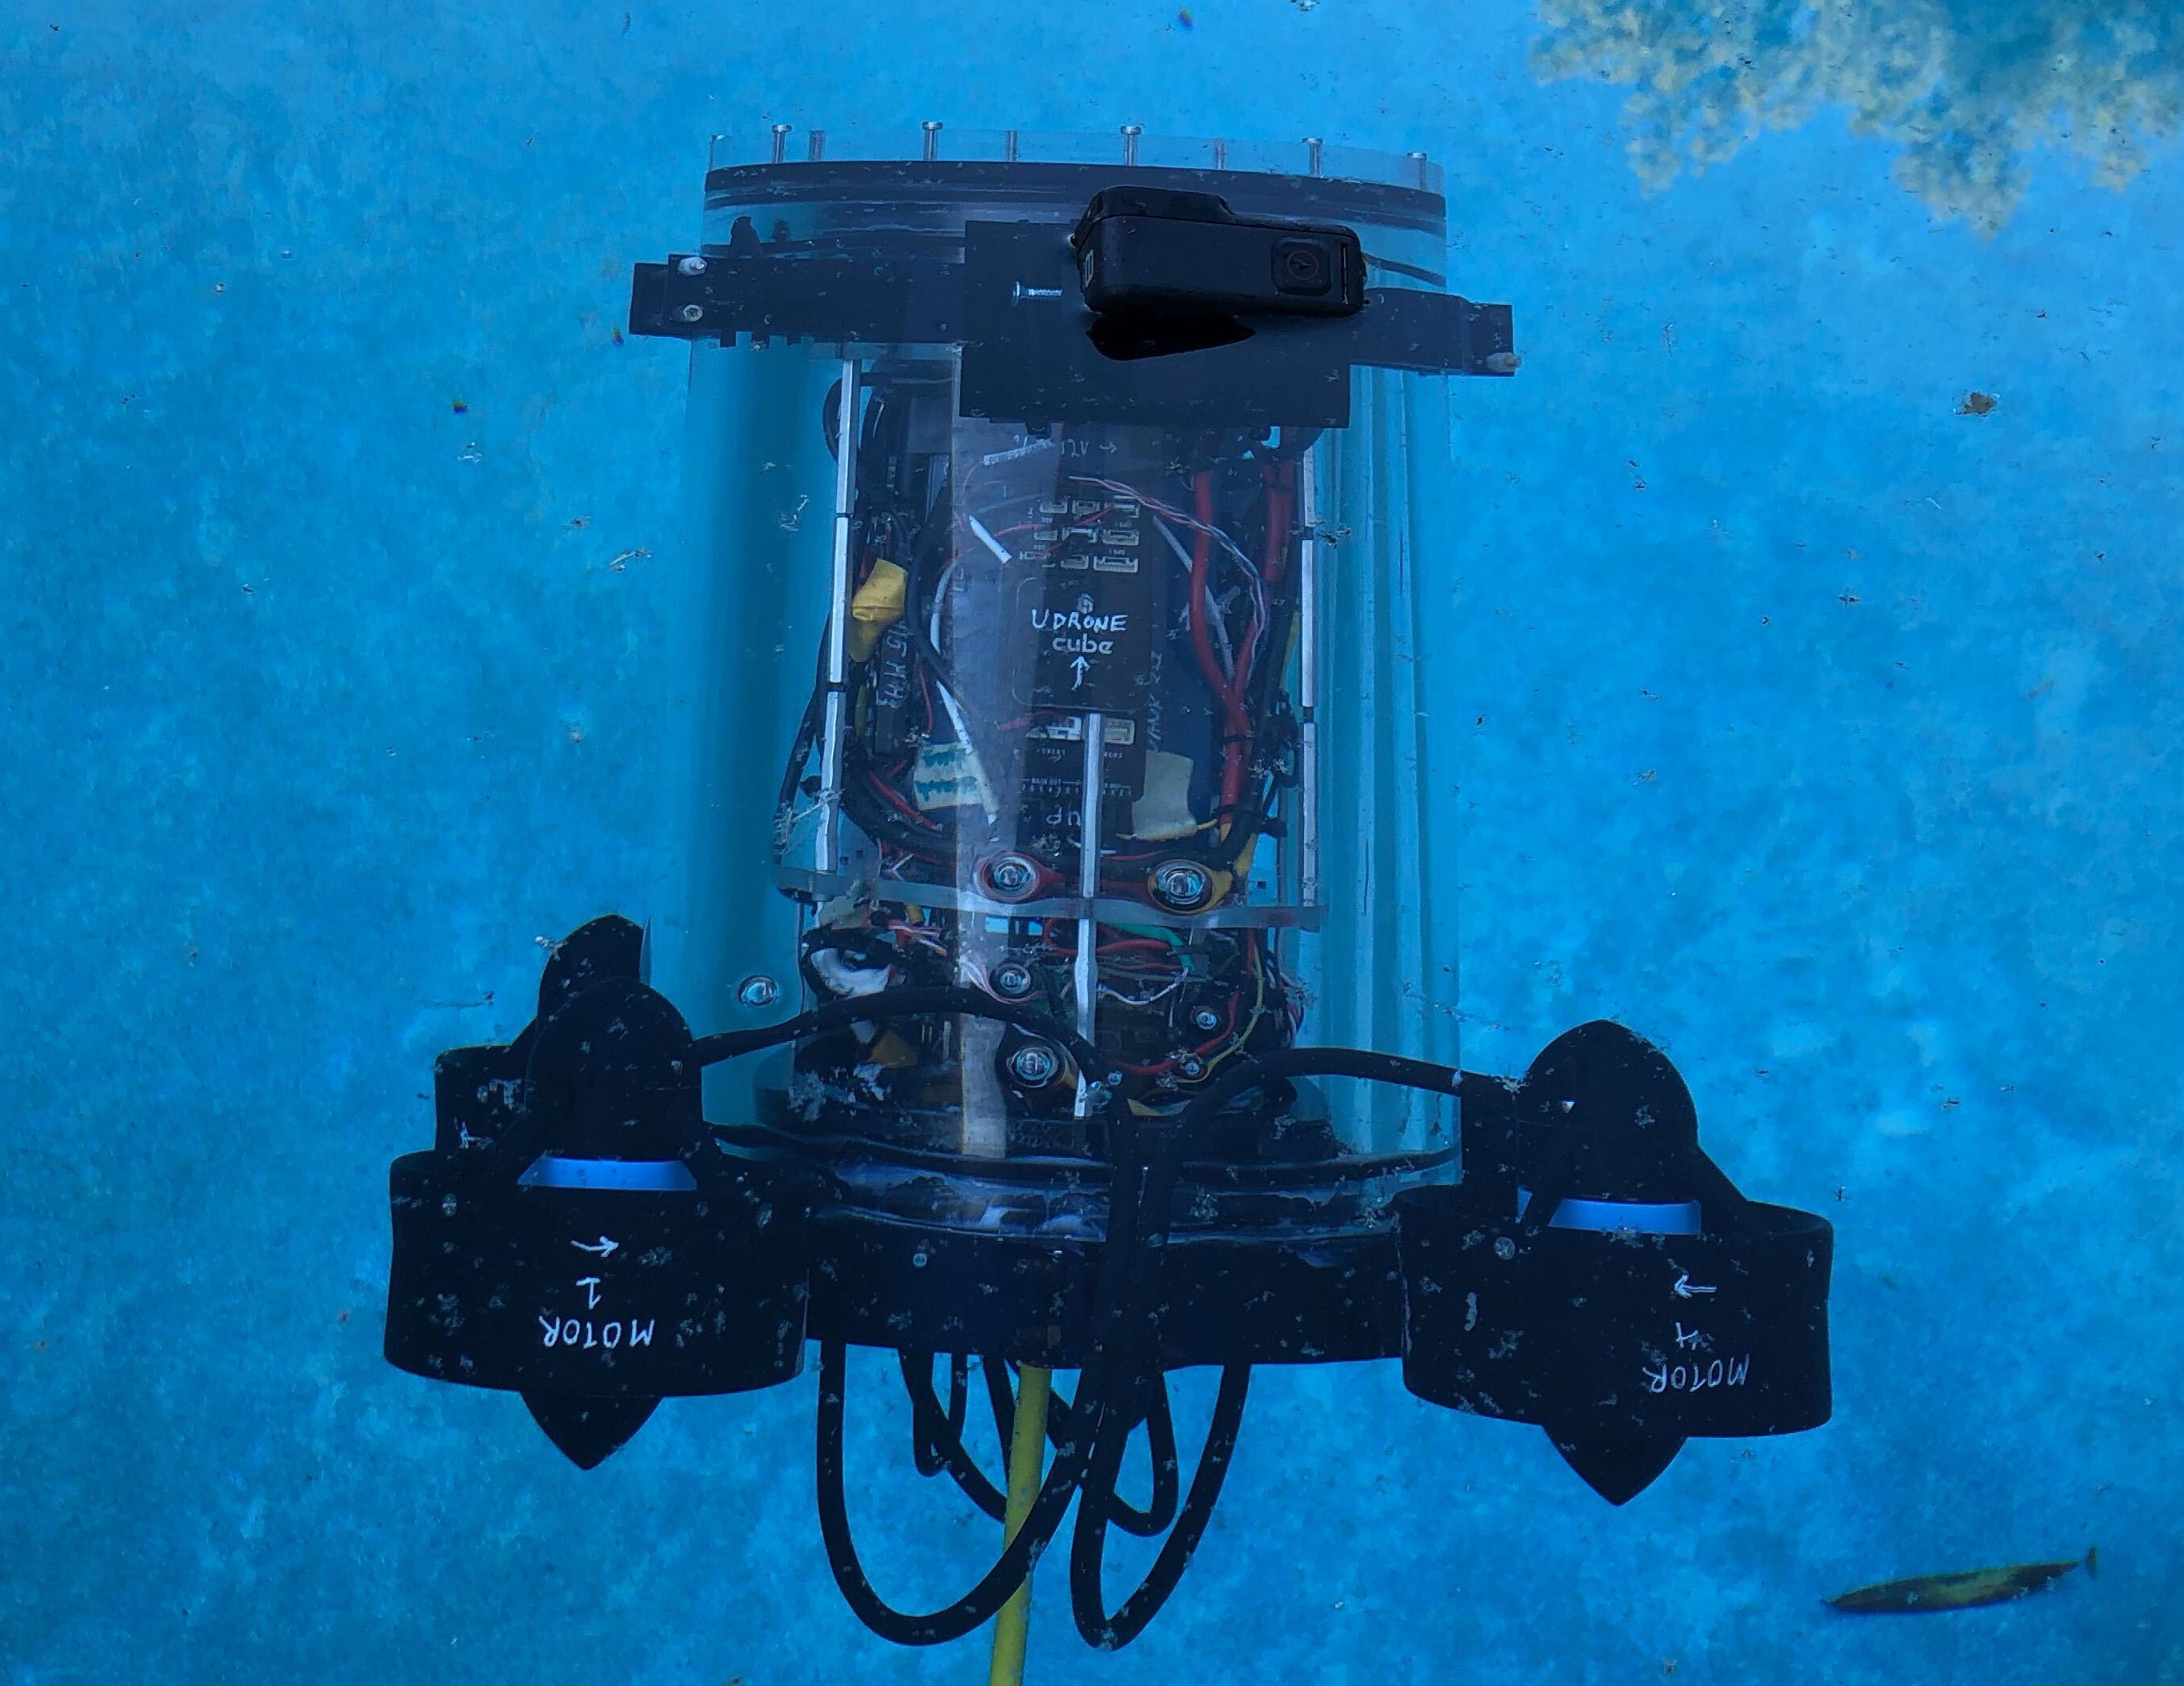
\includegraphics[width=\maxwidth{\textwidth}]{img/drone_pool2.jpg}
\caption{uDrone in Pool Test}
\legend{\emph{Source}: Photo courtesy of Jnaneshwar Das, used with permission.}
\label{pool}
\end{figure}
For all these reasons, the DREAMS lab decided to build a new, customized autonomous underwater vehicle. Based on a motor configuration that mimics that of a quad-rotor aerial vehicle, colloquially referred to as "drones", this vehicle was named the uDrone. This chapter will outline the motivation for developing the uDrone. Subsequent chapters will go through the background of the underwater vehicle world before the uDrone, the technical details of the uDrone system and its development, and a detailed mathematical model of the vehicle dynamics. Lastly, two methods of autonomously controlling the uDrone are explained, evaluated, and compared. 

\section{Thesis Statement}
\begin{center}
    \emph{An autonomous underwater drone testbed that leverages state of the art avionics and machine vision algorithms will enable safe, cost-effective, and time-efficient coral reef exploration and monitoring at a global scale.}
\end{center}
This statement can be broken down to better understand the project goals. Autonomous is defined as being able to operate without direct human control and supervision. Underwater drone is the vehicle itself, emphasizing the setting it is meant to explore. Testbed is a set of software and simulation tools to enable rapid development and testing. State of the are avionics refers to control methodologies and algorithms developed for quad-rotor aerial drones that can be applied to this project. Machine vision algorithms will be used to create and understanding for the vehicle of its surroundings, which is key to enabling autonomy. The uDrone seeks to be safer and less time consuming than the diving being done for related research currently while meeting the budgetary goals. And reef exploration and monitoring is the vehicles ultimate goal and purpose; all the other elements combine to enable this final goal. 

\section{Science Motivation}

GDCS has several ways of obtaining large quantities of imaging data. They contract with Planet satellites and fly an aeroplane fitted with special equipment, known as the Global Airborne Observatory (GAO). These methods have been used to do extensive research on South American rain forests whereas coral reefs are the current "frontier" of research for the GAO. Better imaging and monitoring of coral reefs will enhance researchers understanding of the effects of climate change on reefs and allow for more detailed coral models to be created. 

The immediate goal is to develop a three-dimensional structure of coral reefs that contains full spectral data, from 400 to 800 nm \parencite{gdcs_sat}. This goal is made more difficult by the inherently complex physics of light moving through water. Several methods have been explored to essentially "see through" the water and retrieve the data from the coral alone. In one approach, the inherent properties of the water are used to calculate the effects of the water on the light spectra moving through it \parencite{gdcs_gao}. In another, bottom reflectance data is collected by scuba divers with specialized equipment and used to calibrate the data from satellites \parencite{gdcs_ads}. 

This last method necessitates a human operating in a potentially dangerous environment to collect data. Specifically, Dr. Greg Asner, head of GDCS would use a ADS HandHeld 2 Spectrometer attached to a diver propulsion vehicle (DPV) to collect samples. These data collection trips would last up to four hours and very few researchers have the technical diving capability or constitution to complete them. This was the initial motivation for the uDrone project. Figure \ref{asner} shows the DPV and its use on the reef. 

\begin{figure}[h]
\centering
\subfigure{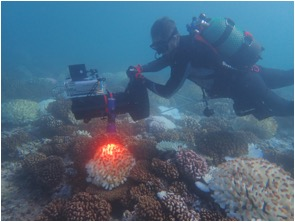
\includegraphics[width=0.49\linewidth]{img/asner.jpeg}}
\subfigure{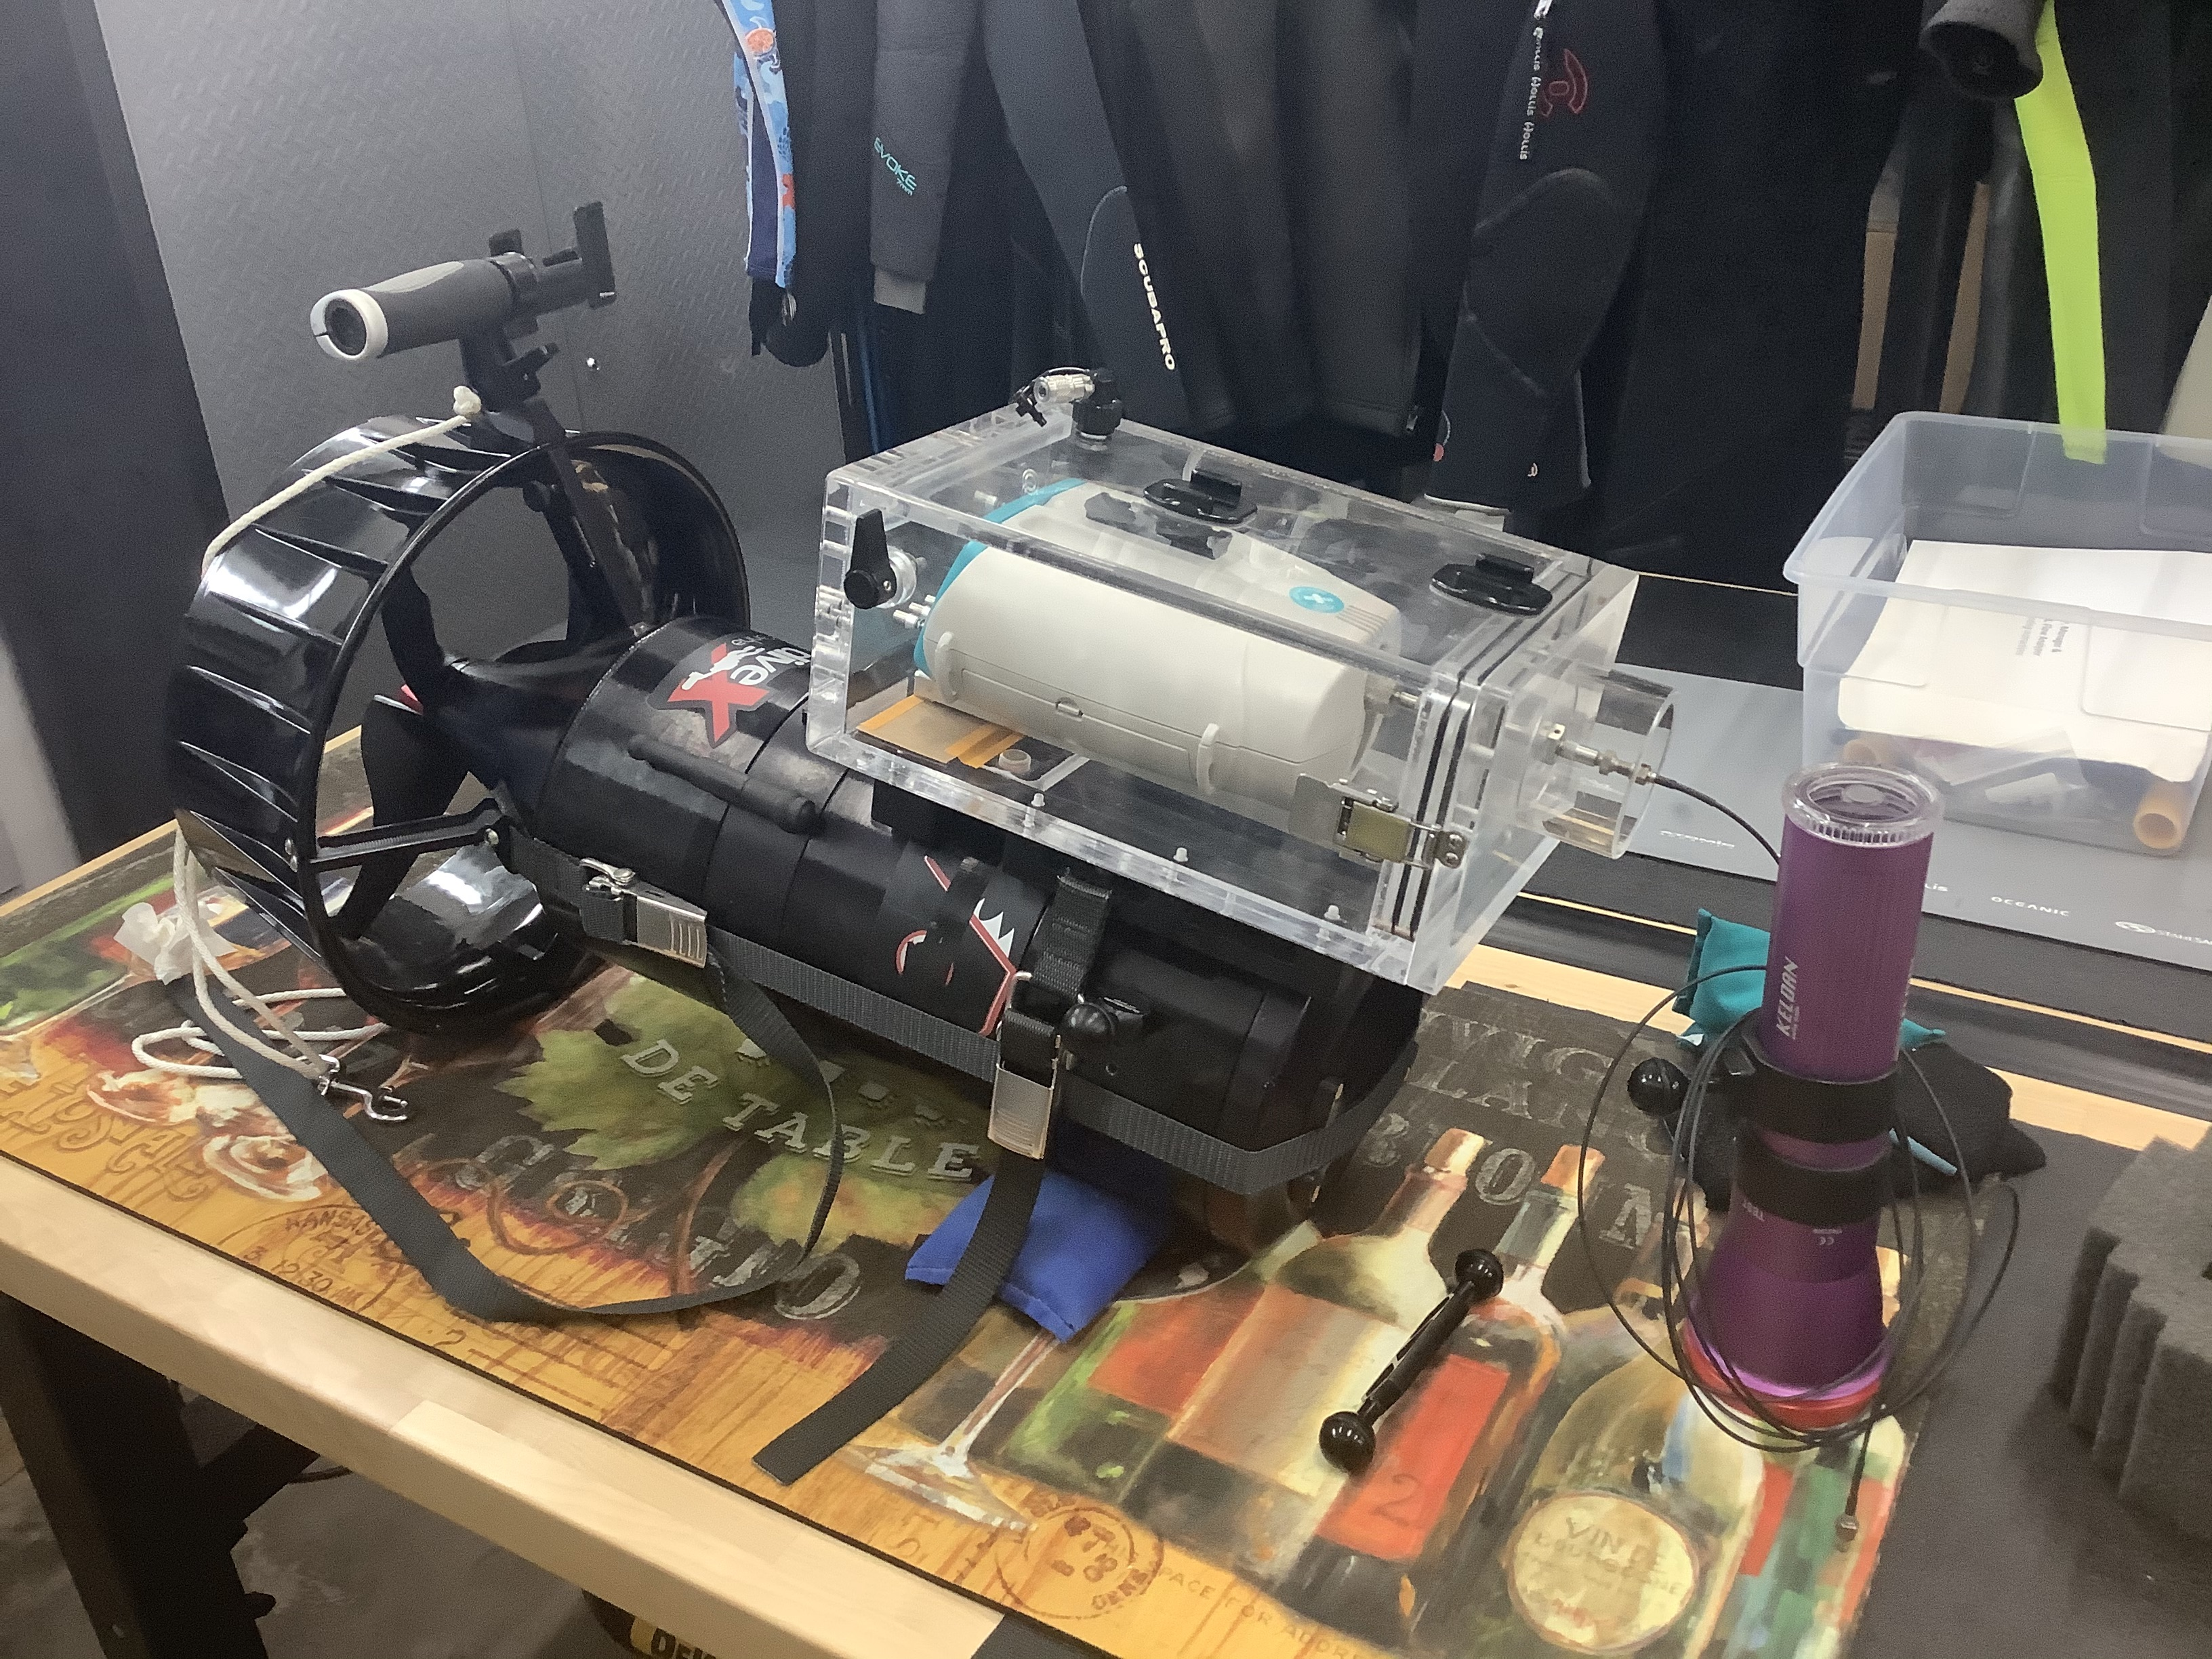
\includegraphics[width=0.49\linewidth]{img/DPV.jpg}}
\caption[DPV Deployed to Collect Reef Data]{Dr. Greg Anser using a DPV for collecting data (left) and the DPV out of water with the sensor attached}
\legend{\emph{Source}: Left photos courtesy of Greg Asner, used with permission.}
\label{asner}
\end{figure}

The risk of death from scuba diving is low, with an estimated annual death rate of 2 deaths per 100,000 recreational scuba divers in the United States. Many of these deaths are due to cardiovascular health and diver errors \parencite{dan}. These risks are mitigated in the scientific diving community by the increased requirements set out by the American Association of Underwater Scientists (AAUS), which require additional training and medical checks \parencite{aaus}. ASU and all associated labs follow these requirements for diving activities.

Dive injury, however, is significantly more common than fatality, with an estimated 15 occurrences per 10,000 dives. While there are many potential avenues for dive injury, including interactions with the marine environment, barotrauma, and gas contamination, one ailment in particular can strike divers at any skill level and is particularly exacerbated by long and repeat dives. This is decompression sickness. Decompression sickness is the second most common type of dive injury, accounting for 27\% of all dive injuries according, to the Divers Alert Network (DAN), the world's largest scuba diving safety association. (Barotrauma is the most common accounting for 41\% of injuries). 

Decompression sickness, or DCS, is caused when gas bubbles absorbed by body tissue at higher pressures underwater are not able to properly “off-gas” or reabsorb. This can cause bubbles to form in various regions of the body. Most commonly this occurs in joints or tissue which can impair motor function and have permanent effects. In some cases a bubble can form in the circulatory system, blocking blood flow, which can be fatal \parencite{dcs}.

In order to reduce the risk of DCS while diving, scuba divers use tools to monitor the dissolved gasses in their system. Historically, this has been done with tables before and after a dive but most modern divers use a dive computer which tracks their gas absorption. This risk can also be mitigated for especially deep or long dives by mixing inert gasses into the breathable air in order to limit the amount of any one gas that gets absorbed.

An AUV, such as the uDrone, can be deployed to totally eliminate the health risks associated with human-based coral reef data collection. This also opens up the possibility of significantly more data to be collected for the existing GDCS projects, along with finding new opportunities for collecting and using reef data. For example, researchers at the University of Hawaii, Hilo are collecting detailed imaging data of coral reefs and using them to create three-dimensional reconstructions of the reef. These reconstructions are then incorporated into other data sets for ecological monitoring \parencite{burns}. The uDrone would allow for more data to be collected with less human health risk as it replaces divers who collect data. 

\section{Engineering Motivation}
While the scientific need inspired its initial creation, the uDrone is useful beyond these specific implementations. It is quickly becoming a testbed for innovation in autonomous underwater navigation within the DREAMS Lab. One thesis has already been written leveraging the system for multi-robot coordination and several others are in the works at this time.

The development of a testbed starts with two parallel tracks: hardware development and software in the loop (SITL) simulation. In the hardware development phase the needs of the vehicle are determined, currently available hardware is specified and sourced, and the vehicle itself is put together. SITL simulation is a method of simulation where all elements of the vehicle are simulated, including the flight controller, the internal computation, the vehicle itself, and the world in which it operates. These tracts combine to a third step: hardware in the loop simulation. In this step the vehicle motion is still simulated in a virtual world, but the flight controller and internal CPU of the actual vehicle interact with this simulation. This step leads to the final step in the chain, which is real world deployment.

\begin{figure}[ht]
    \centering
    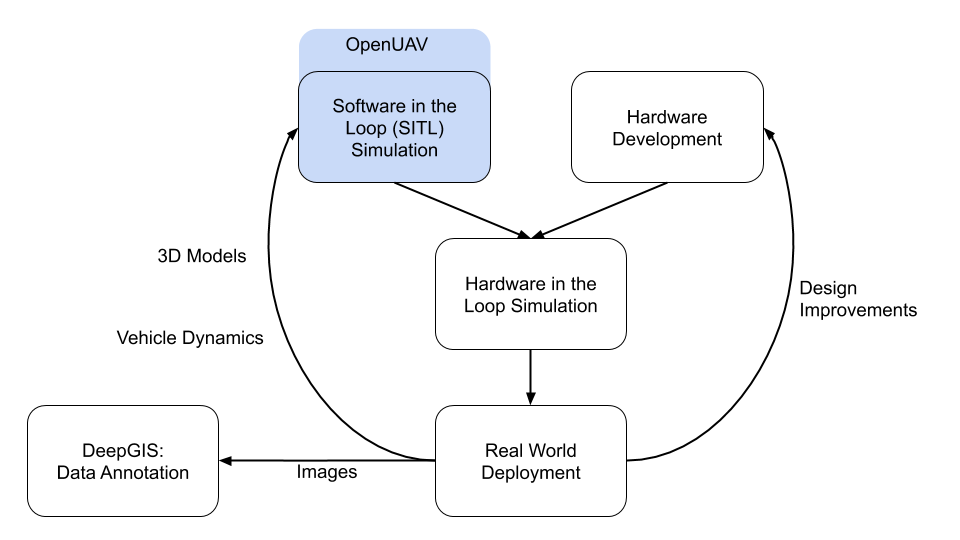
\includegraphics[width=\maxwidth{\textwidth}]{img/testbed.png}
    \caption{The testbed steps and cycle of development}
    \label{testbed}
\end{figure}

This process, illustrated in Figure \ref{testbed}, is not a straight path but a cycle. The real world deployment generates leanings which are put back into the first steps to improve the uDrone. Design improvements are gathered every time the vehicle is put together or deployed. In fact, the vehicle pictured in Figure \ref{3ways} is the third iteration of the internal structure to hold the equipment. The real world deployments also generate more data about the vehicle's dynamics and images collected can be used to create additional 3D reef models. These can be used to make the simulation environment more realistic and accurate. This also feeds nicely into other DREAMS lab projects. The SITL simulation has become part of the OpenUAV stack, a tool for rapid prototyping and remote working. And the images collected from deployment can be fed into DeepGIS, a tool for annotating data for machine learning. 

% This testbed has several benefits for innovation:
% \begin{itemize}
%     \item An existing simulation environment allows for rapid software prototyping. Robotic software developers can focus on writing code, not building simulation environments, and configuring vehicles. 
%     \item Transitioning from simulation to reality is made easier.
%     \item The simulation can be continuously updated as more real-life trials are run with the vehicle. 
% \end{itemize}
    
% Additionally, building a vehicle from scratch is less expensive and easier to maintain than a purchased vehicle. This is because all the components are either off the shelf or built in house. This allows for the efficient acquisition of backup parts. The DREAMS lab team, having intimate knowledge of the vehicle, can troubleshoot and perform maintenance without outside help. Since the cost is low, it is possible to build multiple vehicles and perform swarm activities.

% A good example of similar platform leading to innovation can be seen at Greg Dudek’s Lab at McGill. They AQUA robot was built over 10 years ago and students are still using it today for research \parencite{aqua}. The work has transitioned from hardware to computer vision and autonomous navigation. For example, using this platform a new vision based underwater navigation tool called Nav2Goal was created. In this, the underwater vehicle moves to a goal defined by the user. Along the way, it not only avoids obstacles but also takes paths that bring it near to areas of greater interest. This is particularly useful in coral reefs when a vehicle can decide to follow a path along a coral reef instead of a sandy bottom on its way to its goal \parencite{rtcv}.


% \subsection{Personal Motivation}
% My interest in building the uDrone with the DREAMS Lab at ASU started during my first semester as a Master’s Student in Robotics and Autonomous Systems. I took Prof. Das’ Exploration Systems Design class. My final project for this class was the construction of a boat to start the lab’s stable of aquatic vehicles. For this project, I handled all aspects of construction, system design, assembly, and configuration. This was my first intro to building an autonomous system from the ground up. The boat has been used for several projects in our lab and Prof. Das’ class. After successfully building and deploying this vehicle, and based on my personal experience with scuba diving, I was invited to create the system for an autonomous underwater drone for the lab.

% I started scuba diving at the age of 11. By 15 I had over 100 dives under my belt and was trained as a Rescue Scuba Diver. At 19 I became a certified Scuba instructor. During my undergrad at the University of Michigan, I was one of the leaders of the Human Powered Submarine Team. We designed, built, and raced a submarine powered by a scuba diver inside pedaling bicycle pedals. After school, I volunteered as a Scuba diver at the Shedd Aquarium in Chicago. I proposed to my wife underwater. This is all to say: I have been personally interested in Scuba diving and reef conservation for a very long time. This made me the perfect candidate to leverage my skills in robotics to design a vehicle to help divers get more done.

% Beyond the robotic boat mentioned above, I have a history of building platforms and technology that enable others to achieve more. My first job out of college was at a data center where I developed a novel containerized data center product. This allowed for a drastic decrease in the construction time of data centers while increasing energy efficiency and reliability. Later, I founded several startups with the aim of creating tools and experiences to help. Mm y last and most successful startup created a special type of event that made it easier for strangers to meet and make friends. And immediately before joining ASU for my Master’s, I built a platform for a mortgage company that gave more transparency and power to borrowers in the loan process. This is all to say I am very passionate about building platforms and systems that enable innovation. This, along with the diving, drew me to the challenge of developing the uDrone. 

